\chapter{Requirements on the Simulation Framework} \label{ch:reqs}

In this chapter, I declare the main requirements on the simulation framework. The requirements cover semantics (\autoref{sec:req-semantics}), variable values (\autoref{sec:req-varvals}), back-annotation (\autoref{sec:req-backannotate}), non-determinism (\autoref{sec:req-nondet}), control (\autoref{sec:req-control}), and observation (\autoref{sec:req-observ}). I analyze the requirements, and as a result, present some design decisions and the high-level architecture of the simulation framework (\autoref{sec:sim-architecture}).

The requirement diagram of the simulator is shown in \autoref{fig:reqs}.

\begin{figure}[htbp]
	\centering
	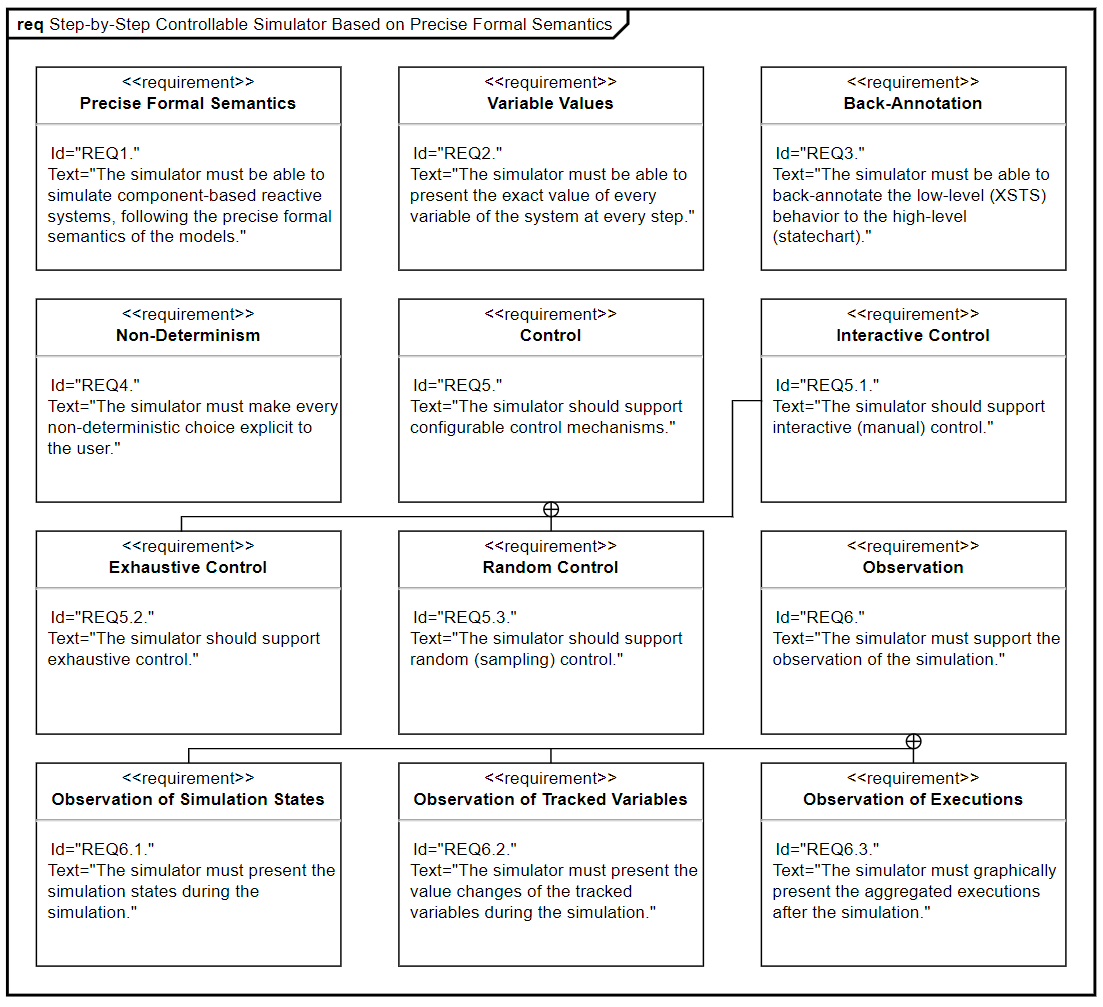
\includegraphics[width=\textwidth, keepaspectratio]{figures/reqs.png}
	\caption{Requirement Diagram of the simulator.}
	\label{fig:reqs}
\end{figure}

\section{Precise Formal Semantics}\label{sec:req-semantics}

\paragraph{REQ1.} \textit{The simulator must be able to simulate component-based reactive systems, following the precise formal semantics of the models.}

Component-based reactive systems can be modeled with Gamma statecharts. Although Gamma statecharts have precise formal semantics, their direct simulation would be hard due to their complexity and high-abstraction level. For formal verification purposes, Gamma provides a semantics-preserving Gamma-to-XSTS model transformation which can be reused for simulation, too. The simulation of XSTS models is easier, due to their lower abstraction level.

In order to follow the exact semantics of XSTS models during simulation, I decided to reuse the model checker infrastructure of Theta, so exactly the same code calculates e.g., the successor states of a state during the simulation and formal verification. With this approach, I can save a lot of unnecessary work and avoid redundant code bases, resulting in easier maintainable software components.

\section{Variable Values}\label{sec:req-varvals}

\paragraph{REQ2.} \textit{The simulator must be able to present the exact value of every variable of the system at every step.}

An important use case of the simulation of behavioral models is that engineers can try out the models they designed. The more details a simulator can give to its user, the more useful it is. It is crucial to always be able to present the simulation state to the user, which, in the case of XSTS models, consists of the exact value of every variable of the system including variables encoding the state of execution (control variables).

The model checking infrastructure of Theta supports the usage of abstraction-based algorithms, such as counterexample-guided abstraction refinement (CEGAR). Abstraction improves the efficiency of model checking, which leads to the support of more complex models. In the case of simulation, efficiency is not a key requirement, so instead of any kind of abstraction, the simulator makes the underlying model checker infrastructure explicitly track the value of every variable.

\section{Back-Annotation}\label{sec:req-backannotate}

\paragraph{REQ3.} \textit{The simulator must be able to back-annotate the low-level (XSTS) behavior to the high-level (statechart).}

Although the simulator simulates the statecharts by generating a semantics-preserving XSTS model from them and simulating the XSTS model itself, it is expected to observe the behavior of the original statechart model, not the XSTS model. To fill the abstraction gap, proper back-annotation could be provided to map every change in the low-level model state to a higher-level behavior, but this is beyond the scope of this work.

Instead, the back-annotation in my work relies on the log mechanism of Gamma. In the high-level statecharts, explicit \textit{log} statements can be defined with a custom string literal. During the Gamma-to-XSTS model transformation, the log statements of every component are transformed into lower-level model elements.

\begin{itemize}
    \item For every \textit{component type}, an XSTS enum type is created, with the same literals as the literals used in the log statements of the component, and a default literal $\mathit{None}$.
    \item For every \textit{component instance}, an XSTS variable is created, with the enum domain corresponding to its component type, and the default value $\mathit{None}$.
    \item For every \textit{log statement}, an XSTS assignment is created, which assigns the enum literal corresponding to the log literal, to the variable corresponding to the component instance. Then, the variable needs to be reset so the default value $\mathit{None}$ is assigned to it.
\end{itemize}

During the simulation of the low-level XSTS model, the value changes of these log variables can be observed to follow the execution of the high-level statechart models.

\begin{example}[Transformation of log statements]
    Consider a component type $T$, and component instances $a$ and $b$ of type $T$. In $T$ (e.g., in the high-level statechart transitions), log statements are defined with string literals $\mathit{log1}$ and $\mathit{log2}$.

    During the Gamma-to-XSTS model transformation, the following log-related model elements are created:
    \begin{itemize}
        \item For component type $T$, an XSTS enum type $D_{\mathrm{log}_T}$ is created with literals $\mathit{None}$, $\mathit{log1}$, and $\mathit{log2}$.
        \item For component instances $a$ and $b$, XSTS variables $\mathit{log}_a$ and $\mathit{log}_b$ are created, with the same domain $D_{\mathrm{log}_T}$. The initial value of every log variable is the default log literal $\mathit{None}$.
        \item E.g., in the case of component instance $a$, the log statement with string literal $\mathit{log1}$ is transformed to XSTS assignments $\mathit{log}_a := \mathit{log1}$, and $\mathit{log}_a := \mathit{None}$.
    \end{itemize}
\end{example}

\section{Non-Determinism}\label{sec:req-nondet}

\paragraph{REQ4.} \textit{The simulator must make every non-deterministic choice explicit to the user.}

In behavioral models, there may be decision points, where the execution can continue in several directions. These decisions are modeled as non-deterministic decisions, which is especially common in the case of reactive systems, where the events coming from the environment are usually modeled as non-determinism.

During simulation, our goal is to provide full control for the user, to be able to control every step of the simulation. Therefore, every non-deterministic decision point must be made explicit to the controller of the simulation.

In XSTS models, there can be non-deterministic decisions inside atomic transitions, too. In order to provide full control for the user, even these inner non-deterministic decisions should be recognized and made explicit. In the given model checker environment, it is not possible to control the inner steps inside an atomic transition, so a pre-process model transformation step (called \textit{splitting}) is required to eliminate internal non-determinism. The splitting algorithm is detailed in \autoref{ch:splitting}.

\section{Control}\label{sec:req-control}

\paragraph{REQ5.} \textit{The simulator should support configurable control mechanisms.}

For different use cases, different control strategies are suitable. At a non-deterministic decision point (i.e., when there are several successor states), the controller of the simulator should select a successor state. Depending on the goal of the simulation and the controller of the simulator (which can be a person interacting with the simulator, or some automatic code), different control mechanisms are required.

\subsection{Interactive Control}

\paragraph{REQ5.1.} \textit{The simulator should support interactive (manual) control.}

When the goal is to let the modeler \textit{try out} their model, they would obviously like to control the simulation themselves. This means, that the simulator is interactive: the decision points are made explicit to the user, who can manually select from the possible successor states, i.e., they can manually select the simulated behavior from the possible ones.

\subsection{Exhaustive Control}

\paragraph{REQ5.2.} \textit{The simulator should support exhaustive control.}

When the goal is to traverse \textit{every possible execution} of a model, interactive control is not practical. Instead, an automated approach is necessary, which -- following some search strategy systematically -- can guarantee the completeness of the traversal.

Note, that the possible executions of a model can be represented as a graph, where the nodes are the states of the execution, and the edges are the possible paths of the execution. In order to explore every possible execution of a model, graph traversal algorithms are suitable, e.g., depth-first search (DFS). This approach is similar to model checking but not for checking a property.

\subsection{Random Control}

\paragraph{REQ5.3.} \textit{The simulator should support random (sampling) control.}

When the goal is to traverse the possible executions of a model, exhaustive traversal is not always an option due to its complexity. Note, that the number of possible executions depends exponentially on the number of non-deterministic decisions in the model. Therefore, in the case of complex models with many non-deterministic constructs (e.g., orthogonal regions), another approach is required to explore the possible executions of a model, not in a complete but in a systematic way.

To achieve this, the simulator can select randomly from the possible successor states at every decision point. In this case, we can increase the completeness of our traversal by increasing the number of simulations.

\section{Observation}\label{sec:req-observ}

\paragraph{REQ6.} \textit{The simulator must support the observation of the simulation.}

It is crucial for the user to be able to observe the simulation -- basically, this is the goal of the simulation.  This observation is required at two levels:
\begin{itemize}
    \item \textit{During the simulation}, the simulation states are presented to the user.
    \item \textit{After the simulation}, the whole execution(s) is/are presented to the user.
\end{itemize}

\subsection{Observation of Simulation States}

\paragraph{REQ6.1.} \textit{The simulator must present the simulation states during the simulation.}

During the simulation, the simulator presents every simulation state to the user. A simulation state is represented by the exact value of every (control) variable of the XSTS model. In the case of interactive simulation, the user can understand the execution and control the decisions based on the presented simulation states. In the case of automated simulation, the presented simulation states can be analyzed and processed programmatically.

\subsection{Observation of Tracked Variables}

\paragraph{REQ6.2.} \textit{The simulator must present the value changes of the tracked variables during the simulation.}

An XSTS model usually contains many variables, which makes the analysis of whole simulation states complex. It is a common use case to track the value of only a few variables, especially the changes in their values. Therefore, the user can track a subset of the XSTS variables, and the simulator explicitly presents their value changes. Observing only the value changes of some tracked variables helps the user to focus only on a specific aspect of the model execution.

Note, that this is especially useful in the case of log variables. If the user tracks the low-level log variables, the presented value changes correspond to the executions of the high-level log statements. This approach allows the user to control the granularity of the observation, by inserting/removing high-level log statements and selecting the tracked low-level log variables.

\subsection{Observation of Executions}

\paragraph{REQ6.3.} \textit{The simulator must graphically present the aggregated executions after the simulation.}

During the simulation, the simulator collects the value changes of tracked variables, and the executions are represented by the sequence of these value changes. After the simulation finishes, the simulator aggregates the executions (if there are more) and presents them graphically.

In the case of a single execution (in interactive mode), no aggregation is necessary. In other cases, the same parts of different executions are merged, in order to emphasize the \textit{differences} between the different executions.

Note, that the granularity of the executions' graphical representation can be controlled by selecting the set of tracked variables. The more variables the user track, the more value changes will be presented and the more insights the user will get about the executions.

\section{Architecture}\label{sec:sim-architecture}

From the above-described requirements, I designed the architecture of the simulator framework which is shown in \autoref{fig:architecture}, an informal figure, showing the main components and interactions of the simulator. It also shows which components satisfy the above-defined requirements  (requirements are marked with gray boxes, satisfy relations marked with dashed lines).

The XSTS splitter splits the original XSTS model into a split one, which the simulator simulates -- it is essential that the model is split because it makes every non-determinism observable and controllable. The core of the simulator is the existing model checker infrastructure of Theta, which is responsible for calculating the possible successor states of the current simulation state. This is wrapped by the simulator, which handles the interactions with the user through a well-defined interface.

The user can control the simulation (at decision points), and the simulator can provide information about different aspects of the simulation to the user. While these pieces of information flow through an interface, different implementations can be used for different control (see \autoref{sec:req-control}) and observation (see \autoref{sec:req-observ}) purposes.

The splitting algorithm of XSTS models and its implementation are detailed in \autoref{ch:splitting}. The architecture and implementation of the simulator are detailed in \autoref{ch:simulator}.

\begin{figure}[htbp]
	\centering
	\includesvg[inkscapelatex=false, width=\textwidth, keepaspectratio]{figures/simulator.svg}
	\caption{Architecture of the simulator.}
	\label{fig:architecture}
\end{figure}

